A continuación, se detallan los diagramas de clases desarrollados para esta fase.

 La carpeta entrenarmodelos contiene cinco archivos, de los cuales dos son responsables de la división del conjunto de datos y su transformación en vectores numéricos densos, también conocidos como embeddings. Los archivos correspondientes son los siguientes: 

\begin{itemize}

\item creando\_dataset.py: Se encarga de la división de los conjuntos de datos en subconjuntos para el entrenamiento, la validación y la prueba, asegurando que cada una de las tres clases esté representada de la mejor manera para el entrenamiento de los modelos. También permite la visualización del estado del conjunto de datos, como el tamaño de secuencias y la bolsa de palabras, para mas detalles ver la figura \ref{fig:uml7}.

\begin{figure}
	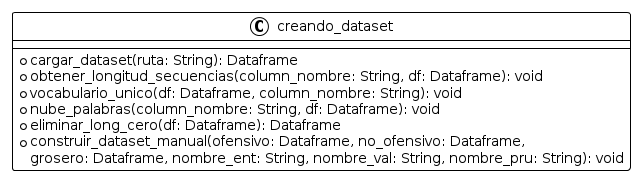
\includegraphics[width=0.65\textwidth]{capitulo5/figuras/fig7.png}
	\caption[Diagrama de clase del archivo creando\_dataset]{Diagrama de clase del archivo creando\_dataset
		\\\textit{Fuente: Elaboración Propia}}
	\label{fig:uml7}
\end{figure}

\item preparar\_datos.py: Recibe el conjunto de datos en formato .CSV mismo que contiene comentarios textuales y sus etiquetas correspondientes. Convierte estos datos a listas para realizar procesos de tokenización, padding, carga de embeddings y procesamiento de embeddings, después de establecer los hiperparametros necesarios como el tamaño máximo de secuencia, el número máximo de palabras y la dimensión de los embeddings, además se crean métodos para el armado de la capa de embedding, compilación, entrenamiento, evaluación y graficación de los modelos, para mas detalles ver la figura \ref{fig:uml8}.

\begin{figure}[h!]
	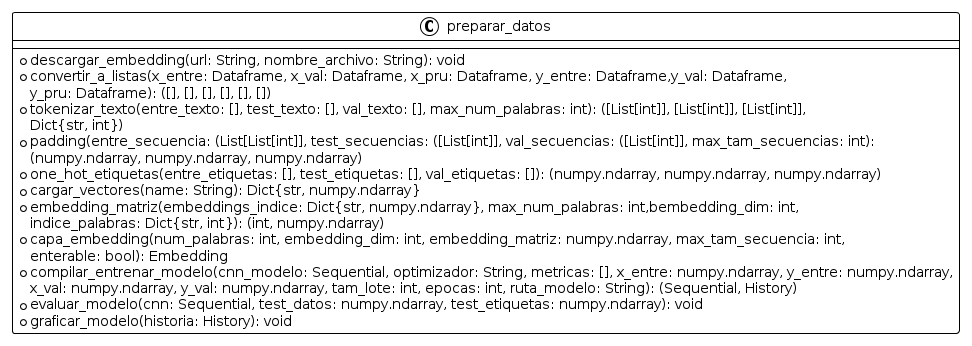
\includegraphics[width=0.95\textwidth]{capitulo5/figuras/fig8.png}
	\caption[Diagrama de clase del archivo preparar\_datos]{Diagrama de clase del archivo preparar\_datos
		\\\textit{Fuente: Elaboración Propia}}
	\label{fig:uml8}
\end{figure}

\end{itemize}

Estos archivos abarcan los procesos de distribución equilibrada de clases, visualización de secuencias, conteo de palabras y creación de la bolsa de palabras del conjunto de datos final, además del manejo de los embeddings. Para la carga de embeddings, se utilizó la versión paga de Colab, debido a la necesidad de usar una mayor capacidad de memoria RAM.
